\documentclass[11pt, oneside]{article}   	% use "amsart" instead of "article" for AMSLaTeX format
\usepackage{geometry}                		% See geometry.pdf to learn the layout options. There are lots.
\geometry{letterpaper}                   		% ... or a4paper or a5paper or ... 
%\geometry{landscape}                		% Activate for rotated page geometry
%\usepackage[parfill]{parskip}    		% Activate to begin paragraphs with an empty line rather than an indent
\usepackage{graphicx}				% Use pdf, png, jpg, or eps§ with pdflatex; use eps in DVI mode
								% TeX will automatically convert eps --> pdf in pdflatex		
\usepackage{amssymb}
\usepackage{hyperref}
\usepackage{subfig}
%SetFonts



\title{Web technologies: Report}
%\subtitle{The fotoquiz}
\author{Youssef Boudiba, Thibaut Deweert, Geatan Boey, Linda de Corte }
\date{}							% Activate to display a given date or no date

\begin{document}
\maketitle
\clearpage

\tableofcontents
\clearpage


\section{Introduction}
You may know the game ?Geoguessr?, where you get to see a random image of Google Street View and you have to guess where you are. The closer your guess is to the real location, the more points you get. Our game has the same idea of guessing a location on a map. Only in our game everyone can upload a picture of a location and a hint. Other people can then guess where the picture is made. They can guess 3 times, every time they lose 20 points and when they ask for an hint they lose half the points.

\subsection{Installation of the project}
\begin{enumerate}
\item Install MongoDB \url{https://www.mongodb.com/download-center?jmp=nav#community} 
\item  Install node.js \url{https://nodejs.org/en/}
\item Install Sails.js \url{http://sailsjs.com/get-started} \\
 npm -g install sails 
\item Start MongoDB service (make sure you point to the database path in the project folder: /data/db) \\ 
mongod --dbpath [Path-to-Project]/data/db
\item Navigate to the project folder and start the Sails.js service
\item The project should be running, visit \url{http://localhost:1337/ }

\end{enumerate}

\section{ The web application architecture}

Photoquiz uses a number of open source projects to work properly:
\begin{itemize}
\item Node.js, an execution environment for event-driven server-siede and networking application
\item Sails.js: popular MVC Framework fore Node.js We chose Sails.js framework because it lets us write everything in the same language and takes over some tasks, for example it automatically sets up an API.
\item AngularJS, this is a very popular JavaScript framework, used to enhance HTML.
\item Express: Fast node.js network app framework
\item MongoDB: this is a a very big noSQL database services. We chose to use it because it is flexible and is easy to use.
\item jQuery: 
\item Bootstrap: An popular HTML, CSS and JavaScript framework, for creating responsive web applications. 
\end{itemize}



\section{Implemented functionalities}
\subsection{User}
\subsubsection{Registering}

A user can register in two ways: the easiest way is by connecting to their Facebook account by clicking on connect to Facebook on the homepage. A popup will open that will ask you to log in, followed by an authorisation page. You will have to authorise this app to log-in.
The other way to register is by making an account. To do this click on the tab register account. Here we have added some restrictions. The -mail field is mandatory and has to be an e-mail adress. The Username has to be filled in, unique and a minimum of 5 characters and finally the password is mandatory and has a minimum of 5 characters.
To check this we use .... (please explain this) \\

\subsubsection{User profile page}
On the user page you will see a few different things. On the left you can see your ranking and the points you've earned. on the right you will see your username, first name, last name and email asdres. You can change your first name, last name and email address. by clicking on edit profile. An pop up will open, edit the fields you want to edit and close the popup to save. \\
On this user page you will also see all the quizes you've made, they are shown in the same grid layout as the quiz overview page. On your own profile page you can also edit your quizes and remove them. Do this by clicking on the buttons below the picture.\\
(Expand if you think that is needed)


\subsection{Quiz}
\subsubsection{ Overview page}
On the Quiz page you can see an overview of all the existing quizes, together with some CSS and bootstrap You will see the picture and the username. Quizes you've done or made yourself are gray-ed out. You can still click on them to see the comments, but you can not guess again. When you click on the picture, you will go to the quiz itself and when you click on the username you will go to the user's profile page. 

\subsubsection{Filtering}
Quizzes can be filtered on location. On the top of the quiz overview page a user can fill in a location and press the 'filter' button. Only quizzes that are within a 30 km range of the given location are then displayed on the page.
It works as follows. Upon pressing the ?filter? button the text from the input field gets transformed to coordinates. This is achieved by using the Google Maps Geocoder which can transform addresses to coordinates. This set of coordinates is then compared with every quiz. For each quiz the distance is calculated between the two, if the distance is shorter then 30 km the corresponding quiz is shown. All this happens on the client side.
If the typed in location is not found, an alert message indicates so. To remove the filter, the user can simply press the ?X?.

\subsubsection{Creating a quiz}
Creating a new quiz can be done by clicking the 'Add' button on the quiz overview page. On the popup that opens the user can fill in some information about his photo quiz. The user can add a personal touch to the quiz by adding a custom message. Eg: ?Visited this museum during my last vacation?. There?s also the option to provide a hint. The player of the quiz can use this hint if he or she has no clue about the location. The message and hint are optional fields. The middle field can be used for uploading a picture and is mandatory. Currently it only supports jpeg images. We use HTML5 form validation on the client side to comply with this restriction. 
After selecting an image and pressing 'next' HTML5 FormData is used to transfer the image file to the server side. The server first reads the exif data from the image and searches for GPS coordinates. The image file is then uploaded to Imgur - an online image host - via the Imgur API. Imgur automatically deletes all exif data, so it is not possible by the players of the game to find the GPS coordinates of die image. When the image is uploaded to Imgur, we save the URL and the delete hash of the image. All this information is stored in the quiz database. \\
On the client side we now get a second popup showing a map with a marker. If the uploaded image included some GPS coordinates then the marker wil be on that position. The user has then the possibility to move the marker to a correct position, if that was not the case yet. If the image had no GPS coordinates in then the user can simply indicate the correct position with the marker. 

\subsubsection{Individual quiz}
When you are on the quiz-page and click on a quiz you will go the quiz page. Here you will see a big map, centered on your location if you've enabled GEO-location. If you've not enabled this the map will center on the VUB. \\
Below the map you can see the picture of which you are searching the location. In the center of the map a marker is shown, to guess the location you have to move this marker and click on guess. \\
You can guess 3 times before you lose. If you guess right in one go you will receive 80 points, overtime you guess wrong you will lose 20 points. You can also ask for a hint, this will cost you half of your points.\\
Al the way below the picture you have a comment section, where you not only can comment on a picture, but also read comments made.
(again extend where needed)

\subsubsection{Search}
In the menu you can also see an search bar. If you fill in a username in this field and click on search you will be redirected to a page where you first get an overview of all the quizes that are made by the users that match te string. This is followed by an overview of all the users that match the string. You can click on the quizes to go to those quiz-pages and click on the usernames to visit the user pages.
(again extend where needed)


\section{Short overview of the requirements} % please think of another title 
\subsection{AJAX}
(still need to be filled in, no idea where this is added)

\subsection{HTML 5}
We have used 4 HTML features in our application

\begin{enumerate}
\item GEO-location, we use this one when you are doing a quiz, it will first center the map on your location.
\item local storage, we use this to store the API secret on the users computer. So they will stay logged in.
\item HTML5 form validation, to make sure the user adds an image when adding a quiz.
\item ????
\end{enumerate}


\subsection{Web service}
\subsubsection{Facebook}
Users have to remember a lot of passwords, to prevent this we have decided to give the user the choice to use their Facebook account to log-in. The moment they chose to use Facebook for logging in we send a request to Facebook, they send back an request to the user for authorisation of the app and when the user authorised we get back the information we need (username and email adress). Now everytime the user wants to log in we will send a request to Facebook in order to check validity.

\subsubsection{Imgur}
For storing the all the images used for the quizzes we used Imgur (http://imgur.com). Using there public available API we can send the images. As return we get a JSON object containing information about the uploaded picture. For this project we only use the link, id and deletehash parameters.

\subsection{Google maps}
We have used Google maps on several occasions.
The first place where we use the google-maps API is when we are filtering based on location. The location the user fills in is send to Google. Google than sends back the gps locations of the location that matches closest with what the user filled in. \\

The next place we use the Google maps API is when a user is adding a picture. We first look if a picture has Exif location data in his or her application. If they have we make a google map with a marker in the center of the location. Otherwise we center on the VUB. The user can than move the marker. when they save we ask the Google maps API to give us the location. \\

And finally we use it when people guess the location, we again make a map with an marker, but this one is based on your GEO-location, if you do not want to share it we will use the location of the VUB for the start point. You can then again move the marker to chose the location. When you think you found the location, you save and we will ask the Google Maps API for the location. We will than do a calculation to see if you were close enough. If not you have 3 chances to guess, again by moving the marker. \\


\subsection{Provide data}
(overview of the API getters and setters)

\section{Conclusion}

\clearpage
\section{Screenshots}
\subsection{Registering}
\begin{figure}[!htb]
\begin{tabular}{cc}
\subfloat[Register: Homepage, log in or register.]{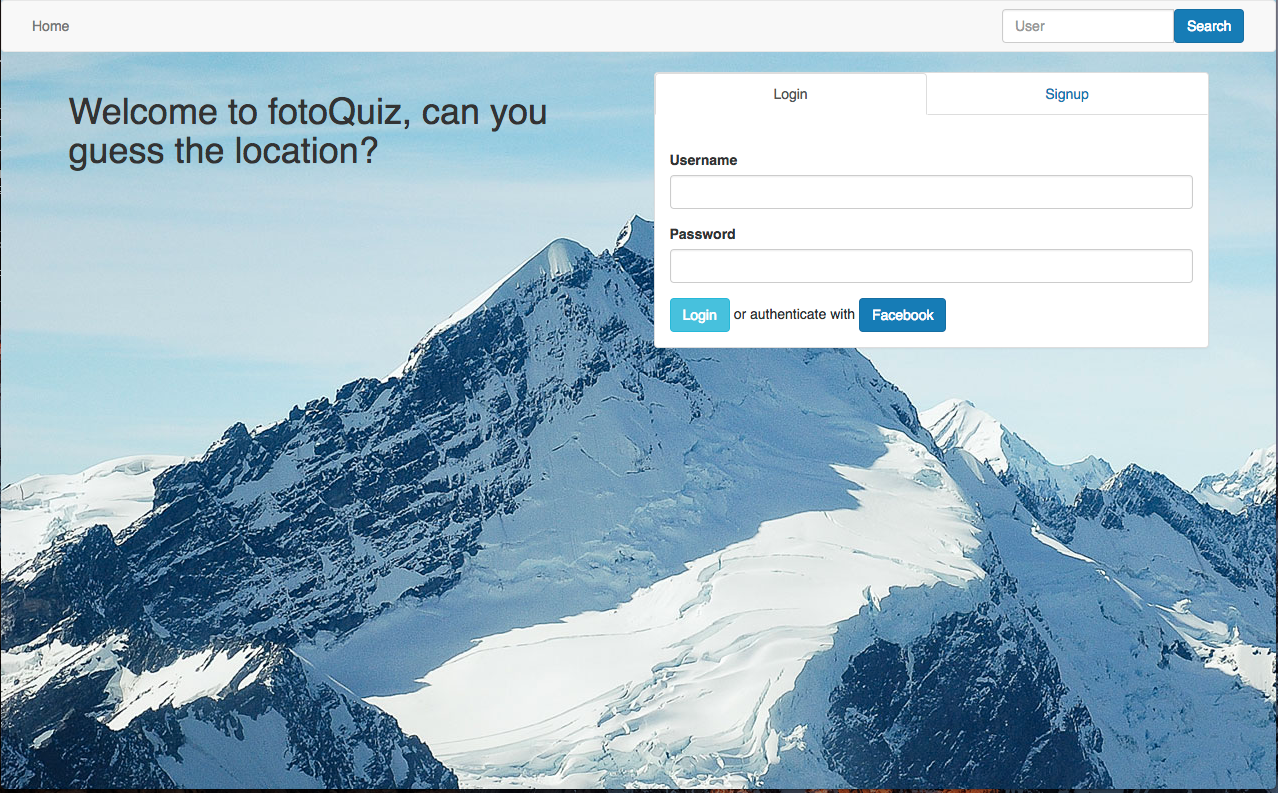
\includegraphics[width=180px]{screenshots/log-in.png}}
\subfloat[Register: User name is taken]{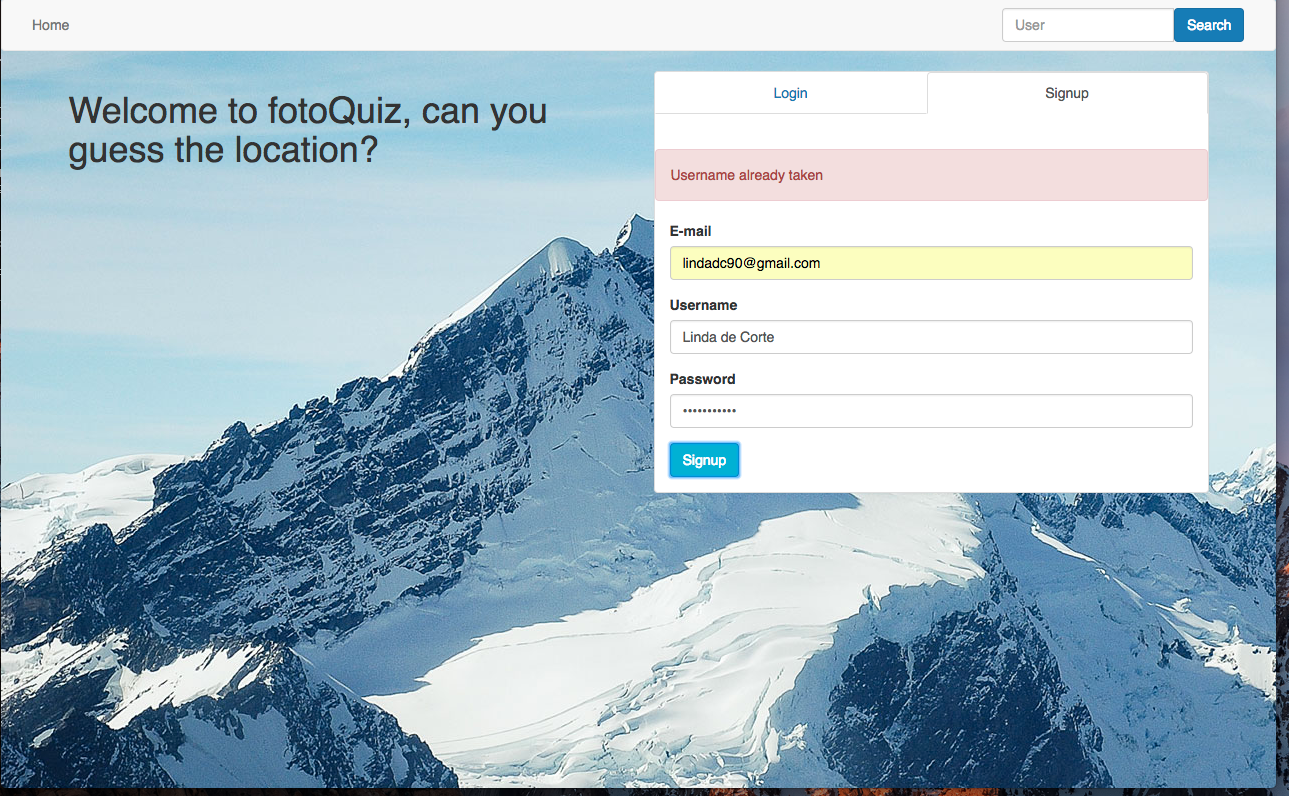
\includegraphics[width=180px]{screenshots/register-username-taken.png}}\\
\subfloat[Register: Username is too short]{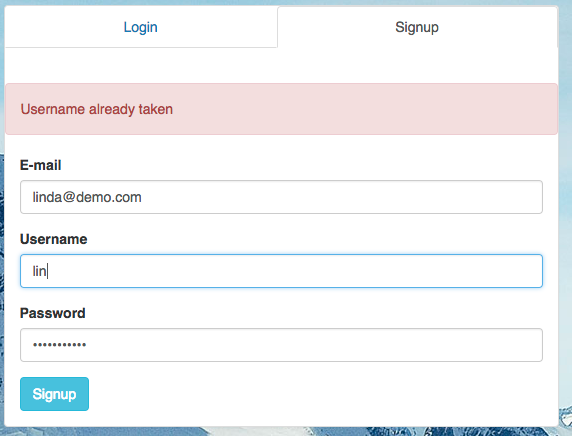
\includegraphics[width=180px]{screenshots/register-short-username.png}}
\subfloat[Register: Not an email adress]{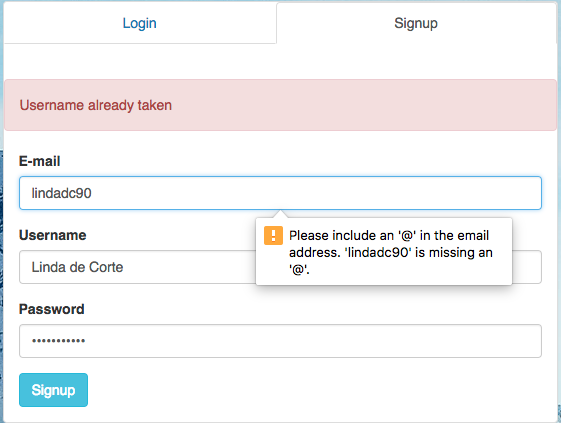
\includegraphics[width=180px]{screenshots/register-no-mail.png}}\\
\subfloat[Register: Password is too short]{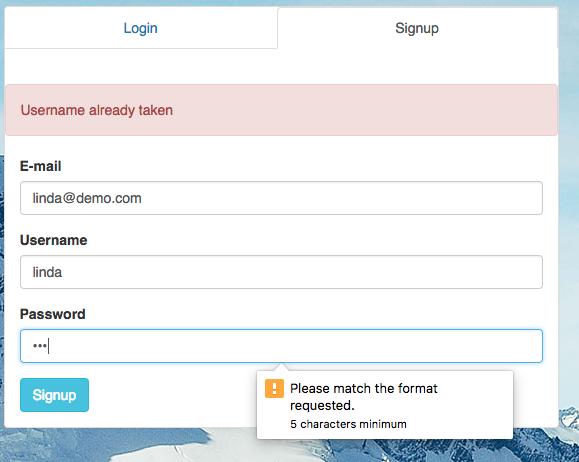
\includegraphics[width=180px]{screenshots/register-short-pw.png}}
\end{tabular}
\end{figure}
\clearpage
\subsection{User profile}
\begin{figure}[!htb]
\begin{tabular}{cc}
\subfloat[The profile page]{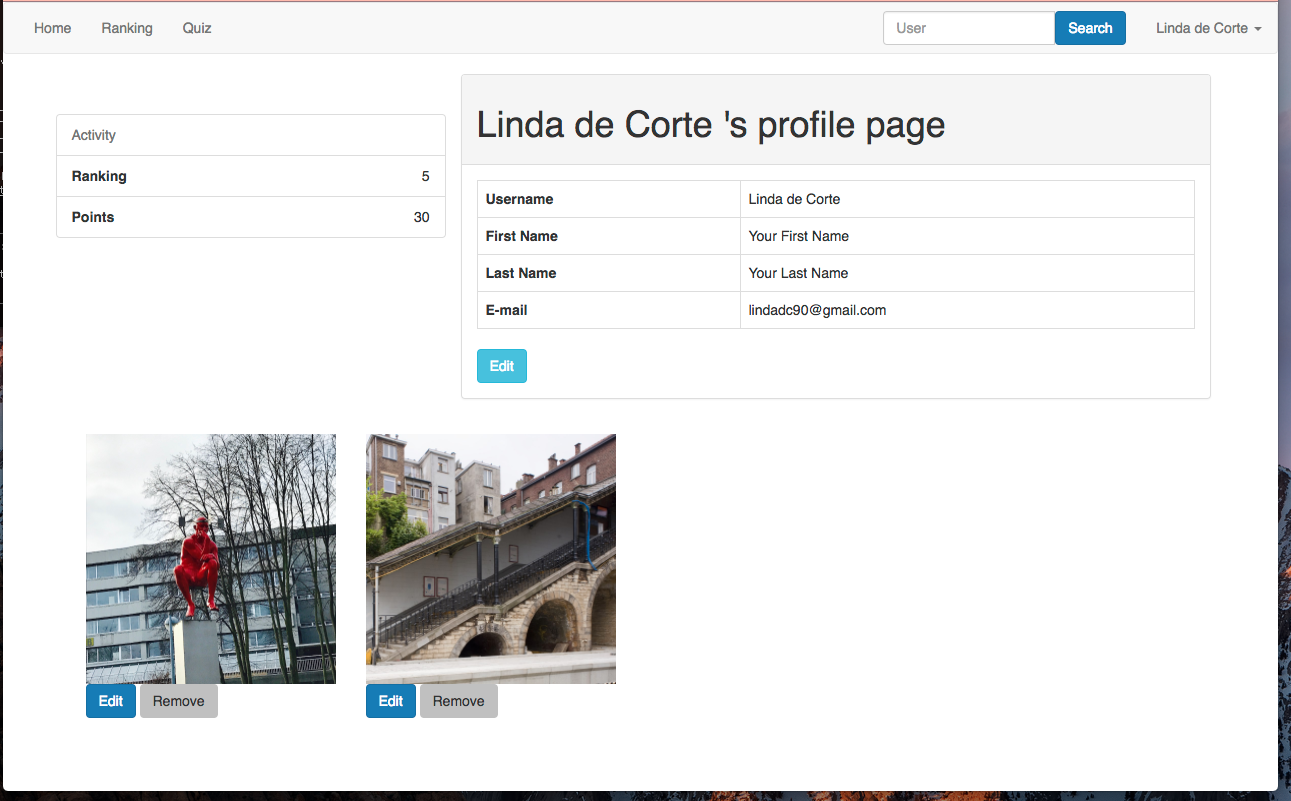
\includegraphics[width=180px]{screenshots/loged-in-profilepage.png}}
\subfloat[Edit profiel]{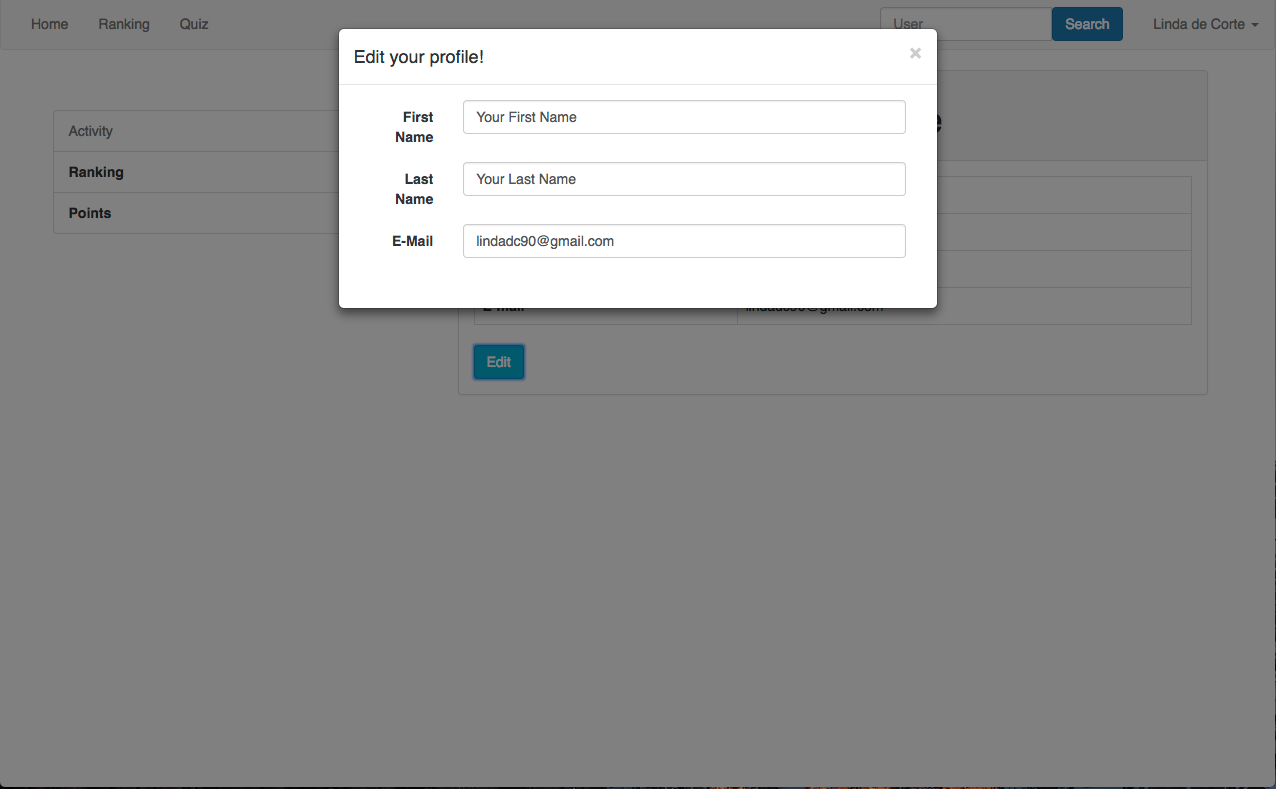
\includegraphics[width=180px]{screenshots/edit-profile.png}}\\
\subfloat[Remove user's quiz]{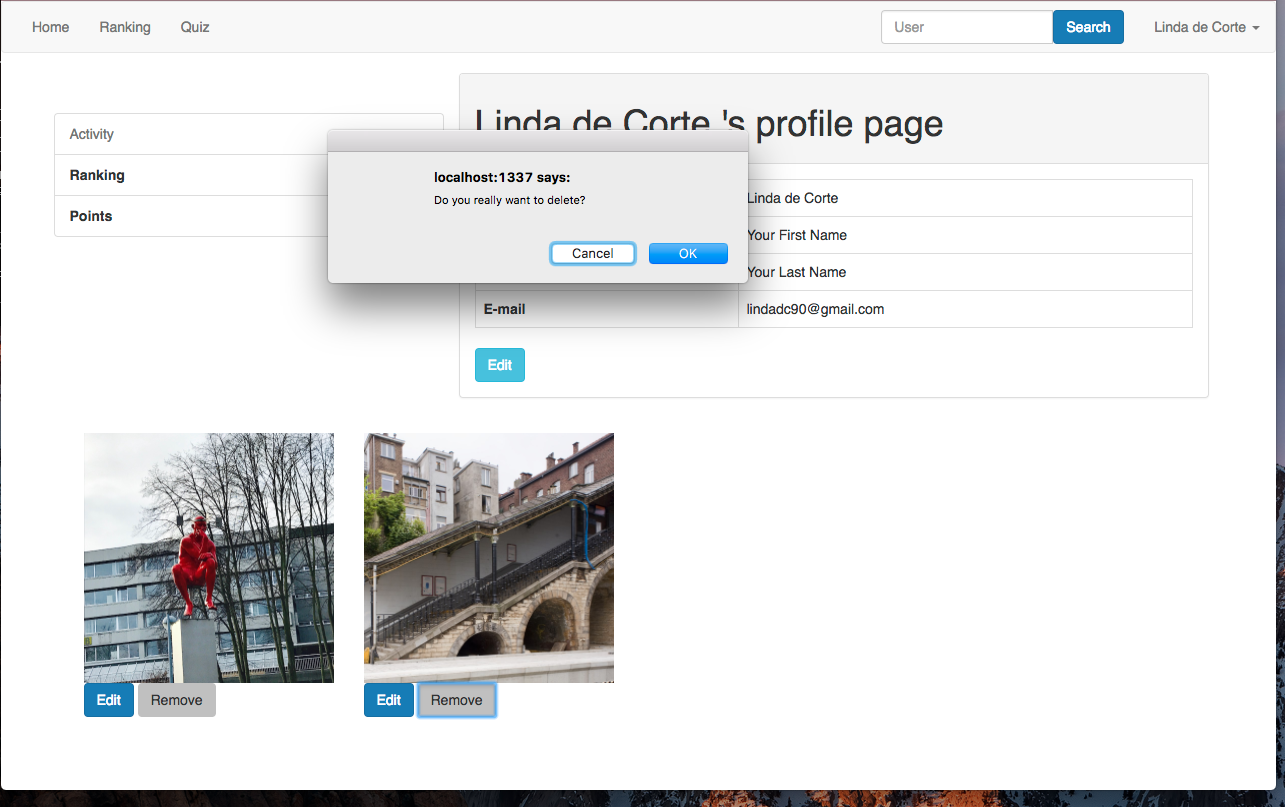
\includegraphics[width=180px]{screenshots/delete-quiz.png}}
\subfloat[Edit user's quiz]{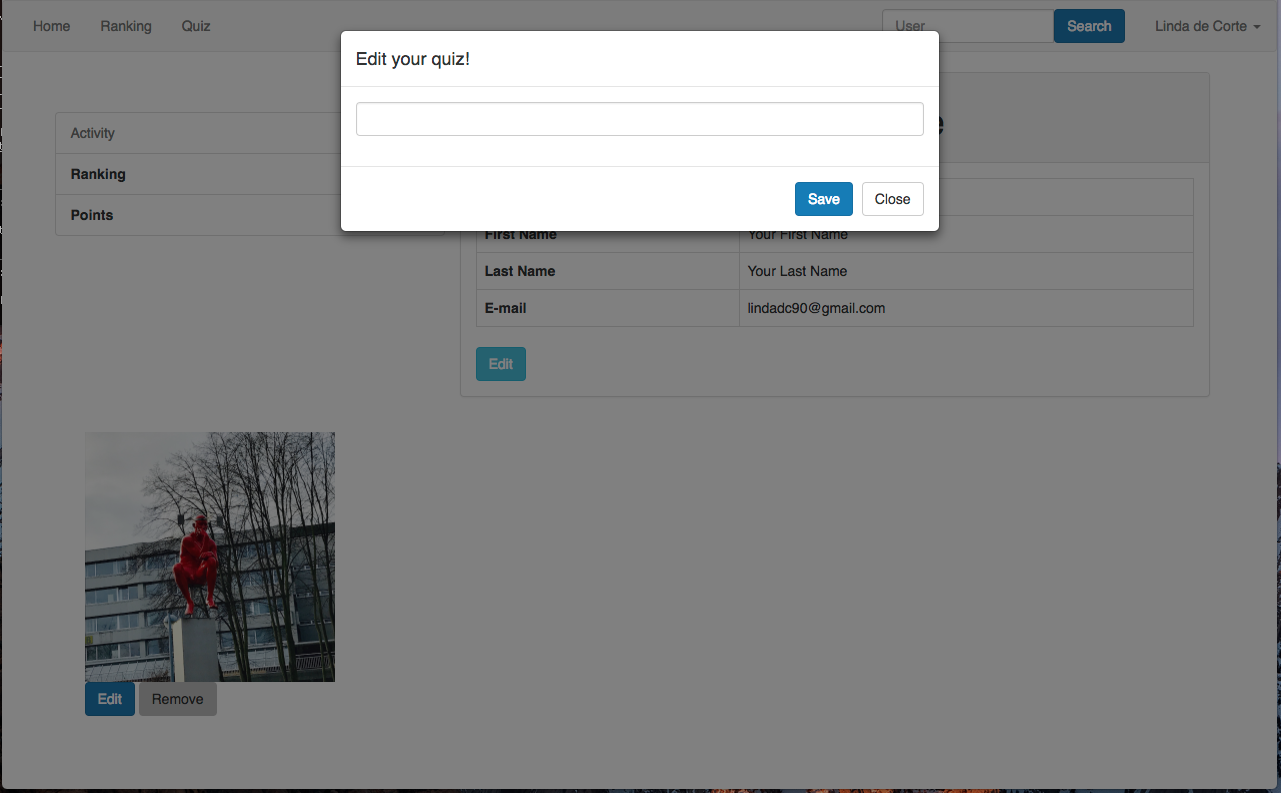
\includegraphics[width=180px]{screenshots/Edit-quiz.png}}\\
\subfloat[Other user quiz]{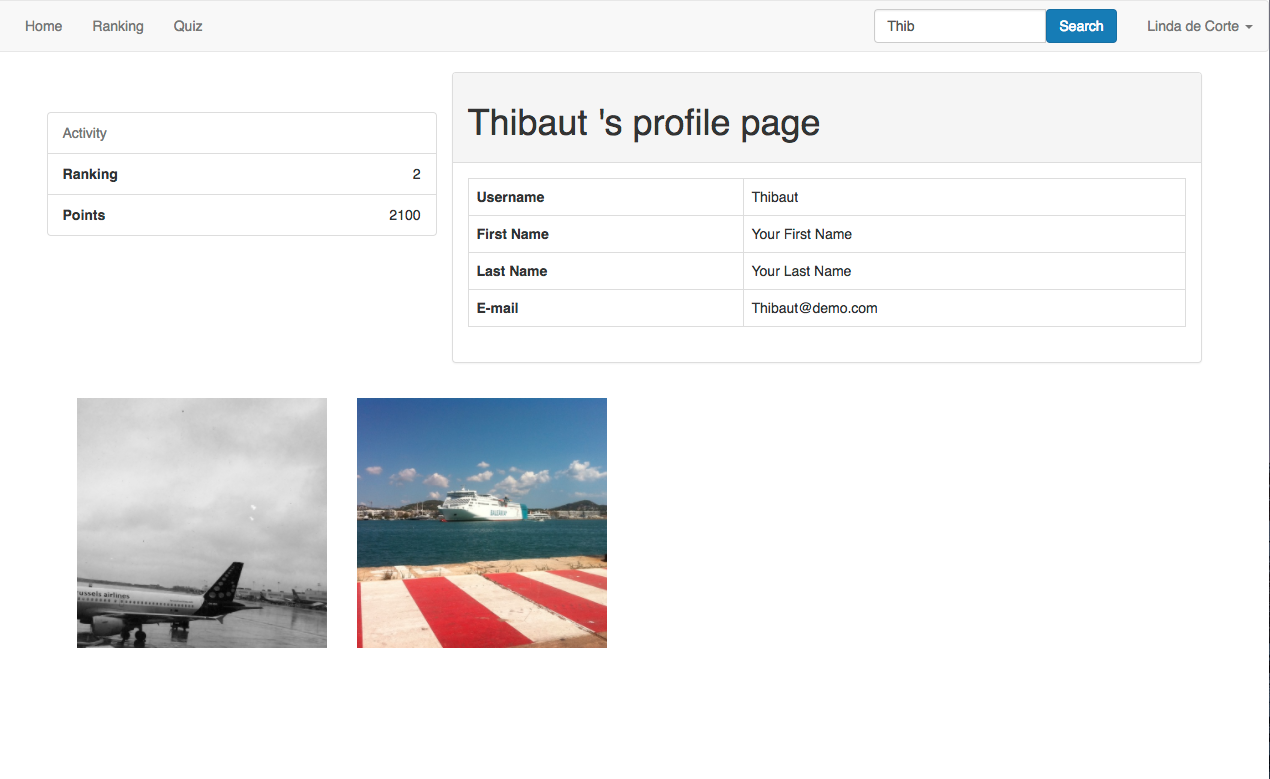
\includegraphics[width=180px]{screenshots/other-user-profile.png}}
\end{tabular}
\end{figure}
\clearpage
\subsection{Quiz}
\begin{figure}[!htb]
\begin{tabular}{cc}
\subfloat[Quiz overview page]{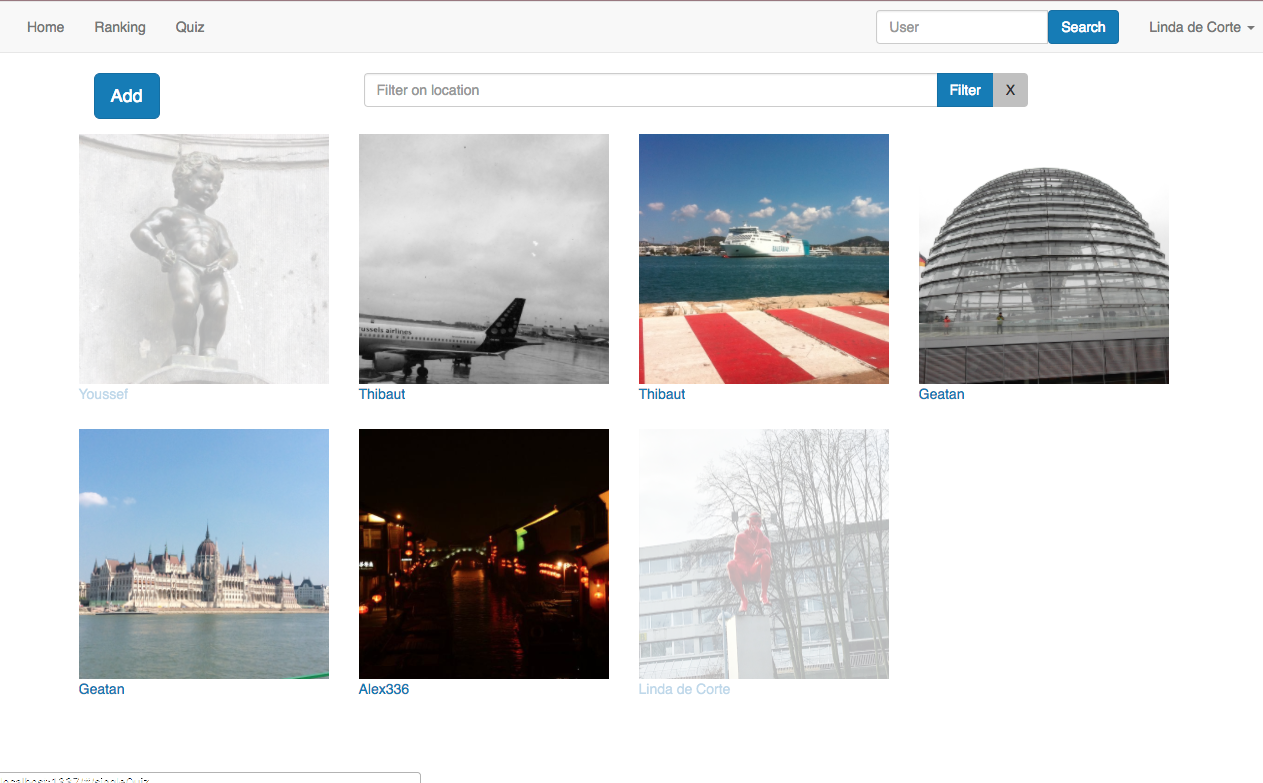
\includegraphics[width=180px]{screenshots/quizpage.png}}
\subfloat[Filter quizes]{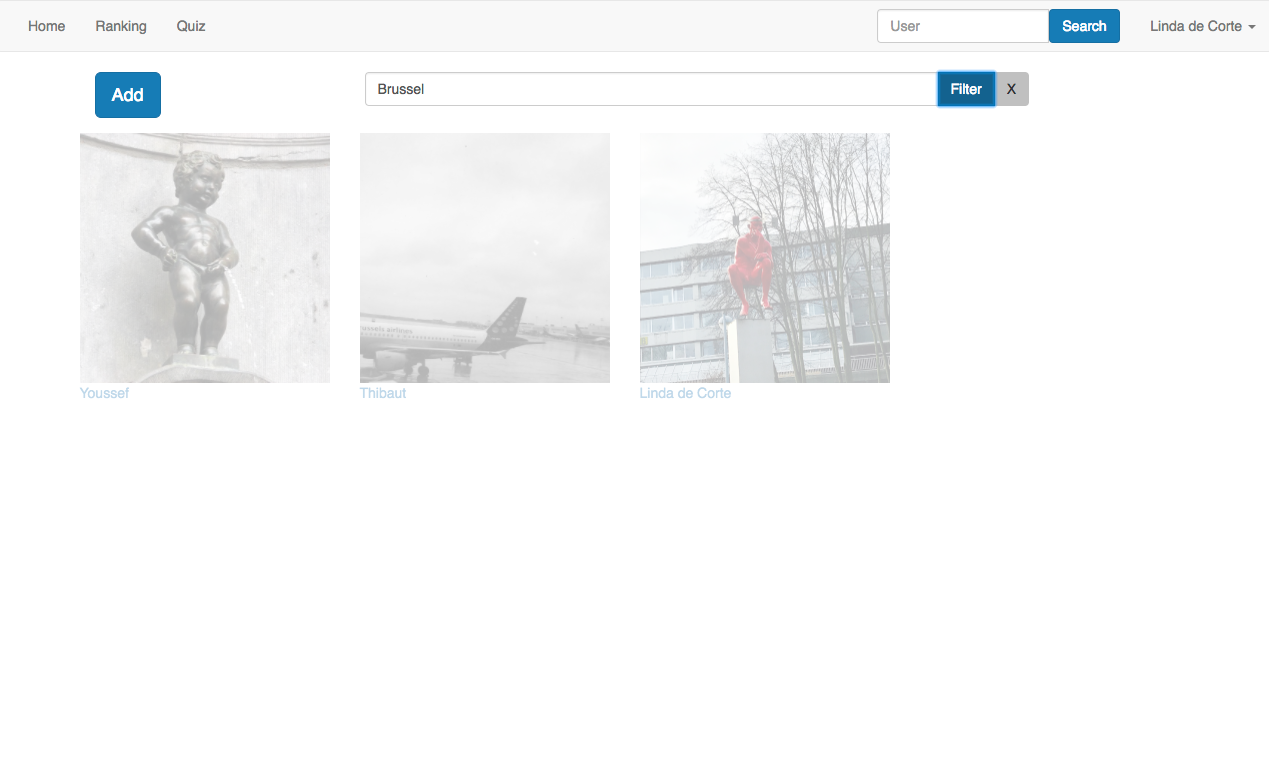
\includegraphics[width=180px]{screenshots/filered-quizes.png}}\\
\subfloat[Add quiz part 1]{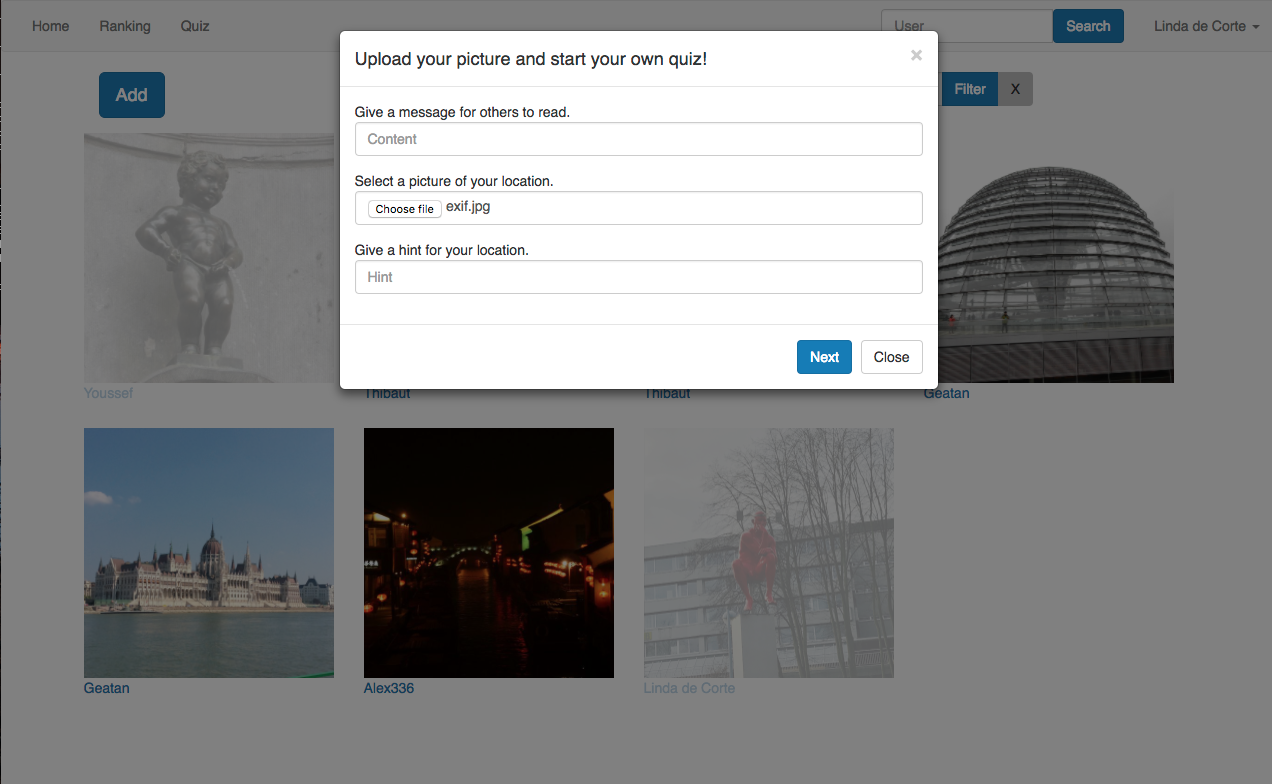
\includegraphics[width=180px]{screenshots/add-quiz-part1.png}}
\subfloat[Add quiz part 2]{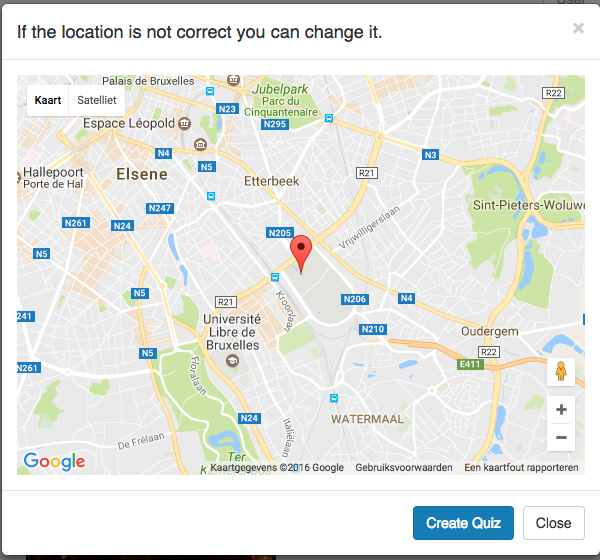
\includegraphics[width=180px]{screenshots/add-quiz-part2.png}}\\
\subfloat[Search User]{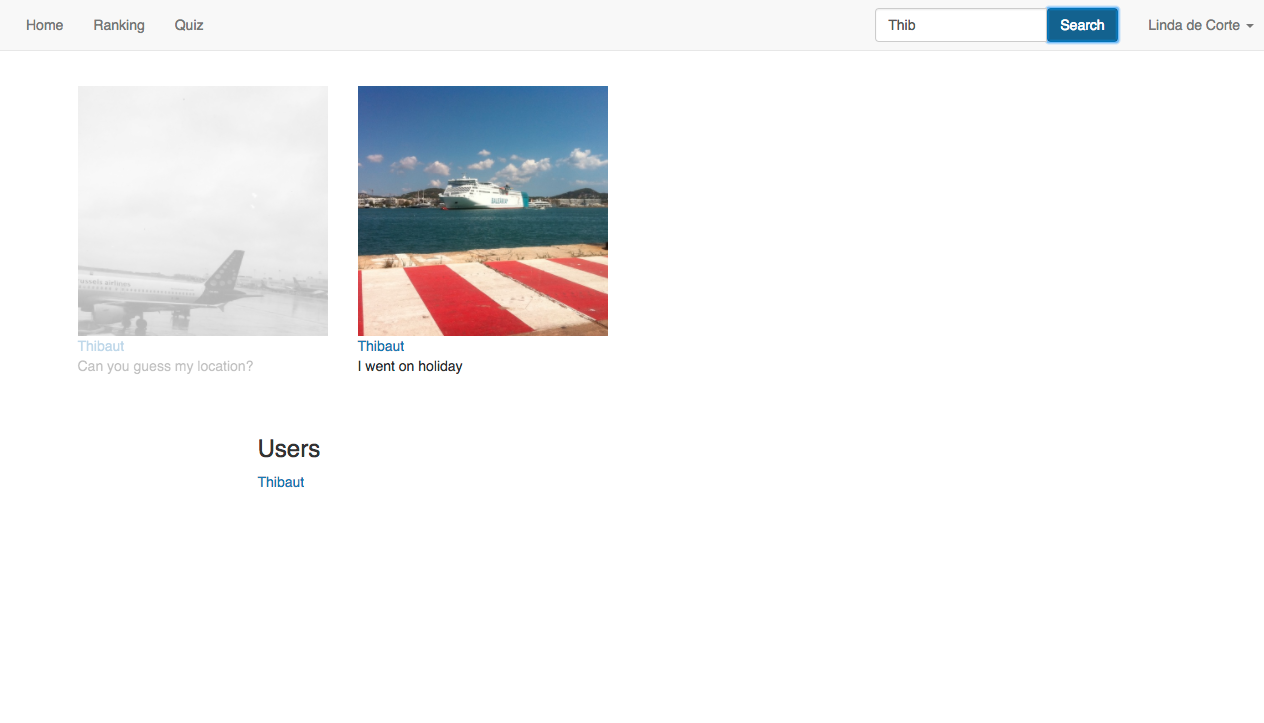
\includegraphics[width=200px]{screenshots/searched-user-2.png}}
\end{tabular}
\end{figure}
\clearpage
\subsection{Indivivual quiz}
\begin{figure}[!htb]
\begin{tabular}{cc}
\subfloat[A individual quiz page]{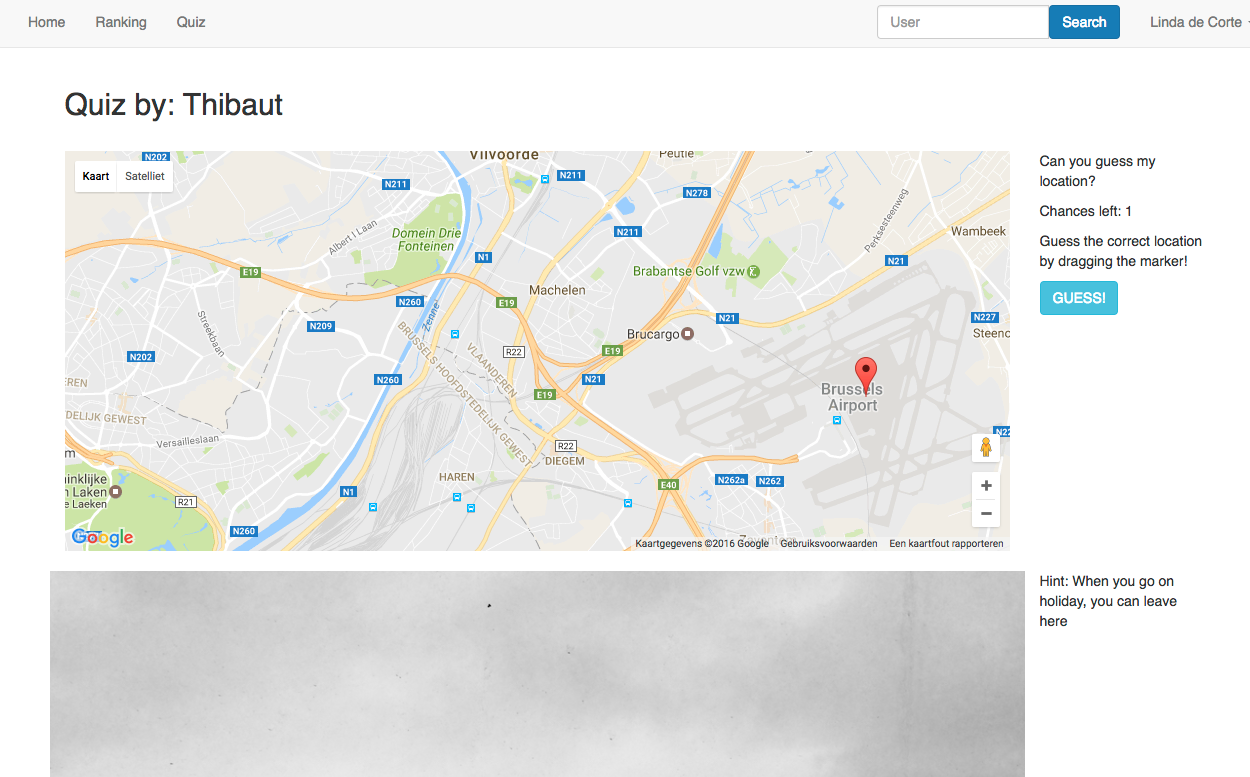
\includegraphics[width=180px]{screenshots/do-quiz.png}}
\subfloat[Comments]{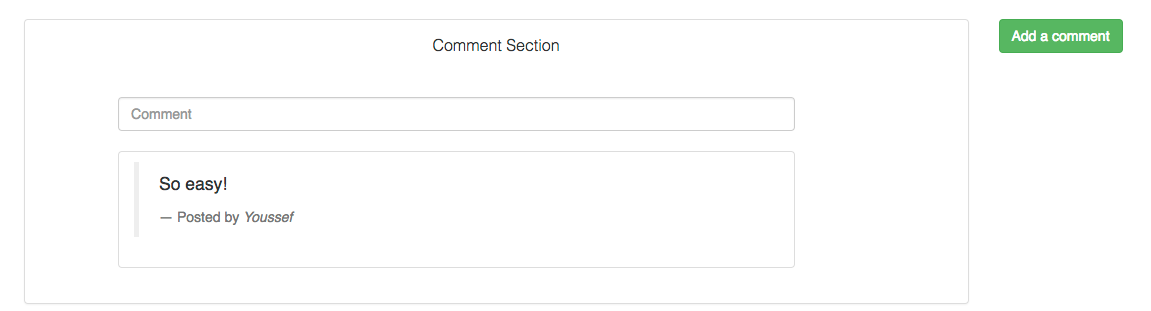
\includegraphics[width=180px]{screenshots/comment-section.png}}
\end{tabular}
\end{figure}



%\subsection{}


\end{document}  